%\documentclass[11pt, twoside, a4paper]{report}
\documentclass[11pt,a4paper]{article}
\usepackage[utf8]{inputenc}
\usepackage{graphicx}
\usepackage{gensymb}

\usepackage{multicol}
\setlength{\columnsep}{1cm}
\setlength{\columnseprule}{1pt}

\usepackage{titlesec}
\titleformat*{\subsection}{\normalsize}

\usepackage{fontspec}
% \setmainfont{Arial}
\setmainfont{Lato}

\usepackage{xunicode}
\usepackage{xltxtra}

\usepackage{amsmath}
\usepackage{amsfonts}
\usepackage{amssymb}

\graphicspath{{./figures/}}
\setcounter{tocdepth}{1}

\usepackage[headings]{fullpage}

\usepackage{fancyhdr}
\pagestyle{fancy}
\fancyhf{}
\fancyhead[LE,RO]{Page \thepage}
\fancyhead[CE,CO]{\leftmark}
\fancyhead[RE,LO]{132-494-F18C-500 Rev.\revisionNumber}

% Setup for Checklist Documents
% ADJUST FORMATING TO SUIT CHECKLISTS
\makeatletter
  \renewcommand{\section}{\@startsection{section}{1}{0mm}%
                                  {-1ex plus -.5ex minus -.2ex}%
                                  {0.5ex plus .2ex}%x
                                  {\normalfont\large\bfseries}}
  \renewcommand{\subsection}{\@startsection{subsection}{2}{0mm}%
                                  {-1explus -.5ex minus -.2ex}%
                                  {0.5ex plus .2ex}%
                                  {\normalfont\normalsize\bfseries}}
  \renewcommand{\subsubsection}{\@startsection{subsubsection}{3}{0mm}%
                                  {-1ex plus -.5ex minus -.2ex}%
                                  {1ex plus .2ex}%
                                  {\normalfont\small\bfseries}}
\makeatother

% REMOVE SECTION NUMBERING
\setcounter{secnumdepth}{0}

% CHECKLIST SECTION DEFINITION
\newcommand{\cSection}[1] {
  \subsection{#1}
  \hrule
  \vspace{.25cm}
}

% CHECKLIST SUBSECTION
\newcommand{\cSubSection}[1] {
  \normalsize{\textbf{#1}}
  \hrulefill \\
}

% CHECKLIST ITEM
\newcommand{\cItem}[2] {
  \normalsize{#1 \dotfill    \textbf{#2}} \\
}

% CHECKLIST COMMENT
\newcommand{\cComment}[1] {
    \\ \textit{#1} \\
}

% Numbered List formating
\renewcommand{\theenumi }{
  \normalsize{\textbf{\arabic{enumi}}}
}



% VARIABLES
\newcommand{\revisionNumber}{00}

\author{132nd vWing}
\title{Aircraft Check-Lists - F/A1-18C}
\begin{document}
  
  \begin{titlepage}
	\begin{center}

        \begin{flushleft}
          \small
          \textbf{\textit{BY ORDER OF THE COMMANDER\\132nd VIRTUAL WING\\}}
        \end{flushleft}

        \begin{flushleft}
        	
\includegraphics[scale=0.4]{./132nd.png}
        \end{flushleft}
        
        \vspace*{-5.6cm}
        
        \begin{flushright}
          \small
          \textbf{\textit{494th VIRTUAL STRIKEFIGHTER SQUADRON}}\\
          \textbf{\textit{DOCUMENT NO. 132-494-F18C-500}}\\
          \vspace*{2.6cm}
          \textbf{\textit{\today}}\\
          \textbf{\textit{POCKET CHECKLIST - F/A-18C HORNET}}\\
        \end{flushright}
        
        \vspace*{0.35cm}
        
        \hrule
       	    
        \vspace{.5cm}
        
        \begin{center}
          \small
          % \textnormal{
          %   ISSUED BY AUTHORITY OF THE CHIEF OF NAVAL OPERATIONS AND UNDER THE DIRECTION OF THE COMMANDER, NAVAL AIR SYSTEMS COMMAND
          % }
          \large{
            DRAFT / WORK IN PROGRESS / UNOFFICIAL DOCUMENT
          }        
        \end{center}

        \vspace{.5cm}

        \hrule

        \vspace{1.5cm}

        \begin{center}
          \small
          \LARGE{
            \textbf{POCKET CHECKLIST - F/A-18C HORNET}
          }
        \end{center}

        \vspace{.5cm}

        \begin{figure}[!ht]
          \centering
          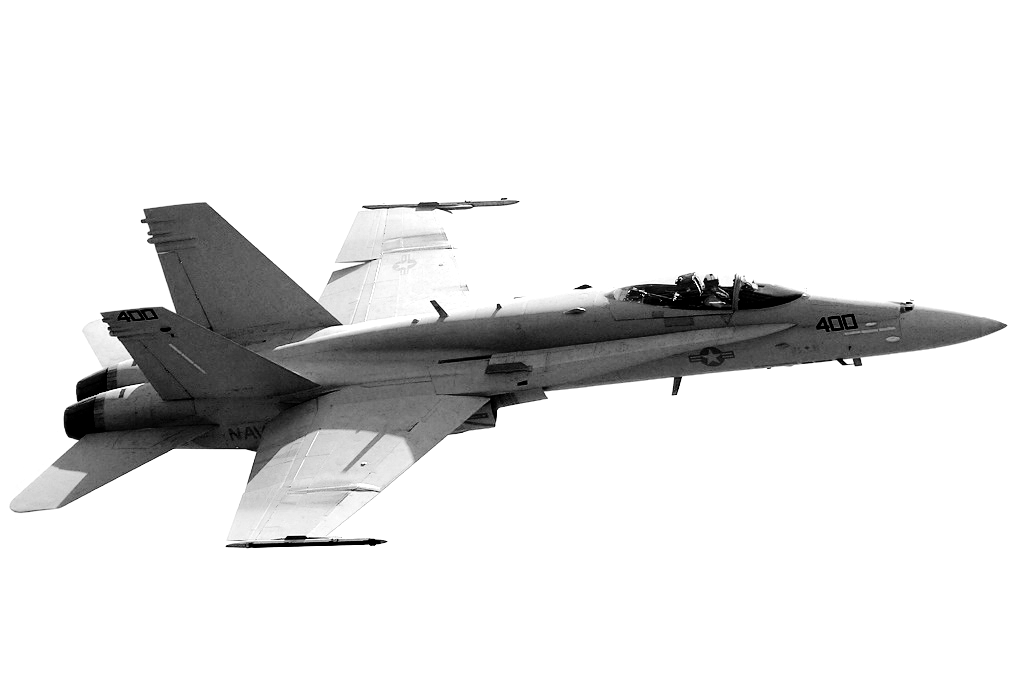
\includegraphics[scale=.3]{./fa18c_illustration.png}
          % \caption{No-fly areas in proximity to the Kutaisi AFB}      
          \label{fig:fa18c_illustration}
        \end{figure}

        \vfill
        
        \normalsize
        % Rev. \revisionNumber
        1.9999
        
	\end{center}
\end{titlepage}

% https://www.overleaf.com/13215577kjhwfcttnsrh#/50849230/
% https://www.sharelatex.com/blog/2013/08/09/thesis-series-pt5.html
  
  \LARGE{
\textbf{NORMALPROCEDURES}
}

\vspace{.25cm}
\hrule
\vspace{.25cm}

\begin{multicols}{2}

\cSection{INTERIORCHECKS}
  \cSubSection{Left Console}
    \cItem{Communications Panel}{SET}
    \cItem{Volume Panel}{SET}
    \cItem{External Tank Switches}{NORM}
    \cItem{Dump Switch}{OFF}
    \cItem{Internal Wing Switch}{NORM}
    \cItem{External Lights}{SET}
    \cItem{Throttles}{OFF}
    \cItem{Parking Brake}{SET}
    \cItem{Landing/Taxi Switch}{OFF}
    \cItem{Anti-Skid Switch(LAND)}{ON}
    \cItem{Anti-Skid Switch(SEA)}{OFF}
    \cItem{Flap Switch}{FULL}
    \cItem{Selective Jettison Knob}{SAFE}
    \cItem{Landing Gear Handle}{DOWN}
    % \cItem{Landing Gear Handle Mechanical Stop}{FULLY ENGAGED}
    \cItem{Canopy Jettison Handle}{FORWARD}

  \cSubSection{Instrument Panel}
    \cItem{Master Arm Switch}{SAFE} 
    \cItem{Altitude Source}{SELECT} 
    \cItem{Attitude Source}{AUTO} 
    \cItem{Clock}{CHECK AND SET} 
    \cItem{IR Coolant Switch}{OFF} 

  \cSubSection{Right Console}
    \cItem{Hook handle}{UP}  
    \cItem{Wing Fold Handle}{SAME AS WING POS} 
    \cItem{Radar Altimeter}{OFF} 
    \cItem{Generator Switches}{NORM} 
    \cItem{Battery Switch}{OFF} 
    \cItem{ECS System}{SET} 
    \cItem{Interior Lights}{AS DESIRED} 
    \cItem{Sensors}{OFF} 
    \cItem{KY-58 Panel}{SET} 


\cSection{ENGINE START}
  
  \cItem{Battery Status}{CHECK}

  \cSubSection{With External Power}
    \cItem{External Power Switch}{RESET} 
    \cItem{Switch 1, 2 and 4}{B - ON (HOLD 3 SEC)}
    \cItem{DDI, HI/MPCD and HUD}{ON} 
    \cItem{Comm 1, 2 and ADF}{AS DESIRED} 
    \cItem{Warning and Caution Lights}{TEST} 
    \cItem{INS}{ENTER WAYPOINTS} 

  \cSubSection{All Starts}
    \cItem{Battery Switch}{ON}
    \cItem{Fire Warning A and B}{TEST BOTH}

  \cSubSection{If APU Start}
    \cItem{APU ACCUM Caution Light}{OFF}
    \cItem{APU Switch}{ON - READY light within 30 seconds}
  
  \cSubSection{If External Air Start}
    \cItem{Bleed Air Knob}{OFF}

  \cSubSection{All Starts}
    \cItem{Engine Crank Switch}{R}
    \cItem{RIGHT Throttle}{IDLE (Min. 15 \% RPM)}
    \cItem{GPWS Voice Alerts}{CHECK}
    \cItem{DDI, HI/MPCD, HUD and UFC}{ON}
    \cItem{EMI/IFEI}{CHECK}
    \cItem{LDDI}{FCS PAGE}
    \cItem{RDDI}{BIT PAGE}

  \cSubSection{Ground Idle}
    \cItem{DESC}{SET}
    \cItem{N2}{63 - 70 \%}
    \cItem{EGT}{190 - 590°C}
    \cItem{Fuel Flow}{420 - 900 pph}
    \cItem{Nozzle}{73 - 84 \%}
    \cItem{Oil Pressure}{45 - 110 psi}

  \cSubSection{If APU or Crossbleed Start}
    \cItem{Bleed Air Knob}{CYCLE 360° TO NORM}
    \cComment{The bleed air shutoff valves close during the fire warning test and the bleed air knob must be cycled thru OFF to NORM with AC power on to reset the valves}
    
    \cItem{Warning and Caution Lights}{TEST}
    \cComment{For a crossbleed start, insure APU switch is OFF and a minimum of 80 \% rpm and 1,900 pph fuel flow}
    
    \cItem{Engine Crank Switch}{L}
    \cItem{LEFT Throttle}{IDLE (Min. 15 \% RPM)}
    \cItem{Engine Crank Switch}{CHECK OFF}

  \cSubSection{If External Air Start}
    \cItem{Bleed Air Knob}{RETURN TO NORMAL}

  \cSubSection{All Starts}
    \cItem{EMI/IFEI}{CHECK}
    \cItem{External Power}{DISCONNECT}


\cSection{BEFORE TAXI}
  \cItem{Radar}{OPR}
  \cItem{INS}{CV, GND or IFA}
  \cItem{OBOGS Control Switch}{ON}
  \cItem{OXY Flow Knob}{ON}
  \cItem{Wingfold}{SPREAD AND LOCK/CHECK}
  \cItem{FCS RESET button}{PUSH}
  \cComment{If wings are folded, verify aileron Xs are present}
  

\cSection{If no reset}
  \cItem{T.O. trim button}{PUSH}
  \cItem{FCS Exerciser Mode}{INITIATE}
  \cComment{Lift FCS BIT consent switch [Y] and push FCS RESET button simultaneously (Hold for a few seconds)}
  % \cComment{Lift FCS BIT [Y] consent switch and push FCS under FCS-MC menu (on RDDI) button simultaneously} \\
  \cItem{APU}{VERIFY OFF}
  \cItem{Hook Bypass}{FIELD/CARRIER}
  \cItem{Fuel}{BIT/SET BINGO}
  \cItem{Attitude Source}{STBY}
  \cItem{Altitude Source}{AUTO}
  \cItem{GPWS}{BOXED}
  \cItem{Mission Data}{ENTER}
  \cItem{Standby Attitude Indicator}{UNCAGE} 
  \cItem{Radar Altimeter}{ON}
  \cItem{Weapons/Sensors}{AS REQUIRED}

%   % \cComment{Enter 3 digit Julian Date and Event Number via UFC}
%   % \cComment{Canopy either full up or full down during taxi}

   \cItem{Ejection Seat}{ARM}

\cSection{BEFORE TAKEOFF}
  \cItem{Canopy}{CLOSED}
  \cItem{IFF}{ON}
  \cItem{INS}{CHECK AND NAV}
  \cItem{Parking Brake Handle}{FULLY STOWED}
  \cItem{MENU Checklist}{COMPLETE}

\cSection{AFTER TAKEOFF}
  \cSubSection{When Airborne}
    \cItem{Landing Gear}{UP}
    \cItem{Flaps}{AUTO}
  
  \cSubSection{10,000 FEET}
    \cItem{Cockpit Altimeter}{CHECK}
    \cItem{Fuel Transfer}{CHECK}
    \cItem{Radar Low Altitude Warning}{CHECK/SET}

  \cSubSection{DESCENT/PENETRATION}
    \cItem{Engine Anti-Ice}{AS DESIRED}
    \cItem{Pitot Heat}{AUTO}
    \cItem{Defog Handle}{HIGH}
    \cItem{Windshield Anti-Ice/Rain Switch}{AS DESIRED}
    \cItem{Altimeter Settings}{CHECK}
    \cItem{Radar Altimeter}{SET AND CHECK}
    \cItem{HUD}{NAV MASTER MODE}
    \cComment{Compare with STBY Flight Instruments and STBY Compass}
    \cItem{NAVAIDs}{CROSS CHECK}
    \cItem{ILS}{ON AND CHANNEL SET}
    \cItem{IFF}{AS DIRECTED}
    \cItem{Weapons/Sensors}{AS REQUIRED}

\cSection{AFTER LANDING}
  \cSubSection{When Clear of Active Runway}
    \cItem{Ejection Seat}{SAFE}
    \cItem{Flaps}{AUTO}
    % \cItem{Landing Gear Handle Mechanical Stop}{FULLY ENGAGED}
    \cItem{T.O. Trim button}{PUSH}
    \cComment{Canopy either full up or full down during taxi}
  
\end{multicols}

\clearpage
  \LARGE{
\textbf{NORMALPROCEDURES}
}

\vspace{.25cm}
\hrule
\vspace{.25cm}

\begin{multicols}{2}

  \cSection{INTERIORCHECKS}
  \cSubSection{Left Console}
    \cItem{Communications Panel}{SET}
    \cItem{Volume Panel}{SET}
    \cItem{External Tank Switches}{NORM}
    \cItem{Dump Switch}{OFF}
    \cItem{Internal Wing Switch}{NORM}
    \cItem{External Lights}{SET}
    \cItem{Throttles}{OFF}
    \cItem{Parking Brake}{SET}
    \cItem{Landing/Taxi Switch}{OFF}
    \cItem{Anti-Skid Switch(LAND)}{ON}
    \cItem{Anti-Skid Switch(SEA)}{OFF}
    \cItem{Flap Switch}{FULL}
    \cItem{Selective Jettison Knob}{SAFE}
    \cItem{Landing Gear Handle}{DOWN}
    % \cItem{Landing Gear Handle Mechanical Stop}{FULLY ENGAGED}
    \cItem{Canopy Jettison Handle}{FORWARD}

\end{multicols}

\clearpage
  \LARGE{
\textbf{CASE 1 - CARRIER RECOVERY}
}

\vspace{.25cm}
\hrule
\vspace{.25cm}

\begin{multicols}{2}

  \cSection{INBOUND - 10 NM}
    \cItem{COMM1 or COMM2}{CONTACT CATCC}
    \cComment{Join Port Holding Pattern as instructed}

  \cSection{HOLDING PATTERN - 5 NM CIRCLE}
    \cItem{Altitude}{AS INSRUCTED (Min. 2000 ft)}
    \cItem{Airspeed}{250 KIAS}
    \cItem{Hook}{DOWN}
    \cItem{Anti-Skid Switch}{OFF}
    \cItem{Hook Bypass}{SEA}
    \cComment{Depart Holding Pattern 30° opposite BRC heading (210° from BRC) - AFT of ship's beam}

  \cSection{Initials - 3 NM AFT}
    \cItem{Altitude}{800 FT}
    \cItem{Airspeed}{350 KIAS}
    \cItem{Hook}{CHECK DOWN}
    \cItem{LDDI}{HUD}

  \cSection{Break}
    \cItem{Speed Brake}{EXTEND FULLY}
    \cItem{Altitude}{KEEP 800 FT}
    \cComment{Rule of Thumb: Match Gs according to 1/100 of Airspeed during deceleration in order to arrive at On-Speed AOA on roll-out (350 KIAS => 3,5 G)}

  \cSection{ABEAM (180) - 1.2 TO 1.5 NM}
    \cItem{Trim}{AS REQUIRED}
    \cItem{Altitude}{600 FT}
    \cItem{Speed}{ON SPEED AOA}

    \cSubSection{Below 250 KIAS}
      \cItem{Landing Gear}{DOWN AND LOCKED}
      \cItem{Flaps}{FULL}
      \cComment{Target speed approximatly 140 KIAS}

    \cSubSection{Turn to final}
      \cItem{Position}{ABEAM LSO PLATFORM}
      \cItem{Angle of Bank}{30°}
      \cItem{Rate of Decent}{200 - 300 FPM}
      \cItem{Speed}{ON SPEED AOA}

  \cSection{Aft (90) - 3/4 NM}
    \cItem{Altitude}{450 FT}
    \cItem{Rate of Decent}{500 fpm}
    \cComment{Maintain optimum AOA, and a 30° AOB}

  \cSection{IN THE GROOVE}
    \cItem{AOA}{CHECK}
    \cItem{Rate of Decent}{CHECK}
    \cItem{Ball Call}{CALLSIGN TYPE FUELSTATE}
    \cComment{"Thunder 204, Hornet, Ball - Three Point Five"}



\end{multicols}


% ILLUSTRATIONS

\clearpage
  \LARGE{
\textbf{RADIO PRESETS - COMM 1 and COMM 2}
}

\vspace{.25cm}
\hrule
\vspace{.25cm}

\begin{multicols}{2}
  \cSection{COMM 01 - V/UHF}
      \cItem{1 - Internal \#1}{233.000}
      \cItem{2 - Internal \#2}{232.500} 
      \cItem{3 - Internal \#3}{232.000} 
      \cItem{4 - Internal \#4}{235.250} 
      \cItem{5 - Internal \#5}{244.750} 
      \cItem{6 - Internal \#6}{232.250} 
      \cItem{7 - Tanker A}{230.750} 
      \cItem{8 - Tanker B}{235.500} 
      \cItem{9 - Inflight Report Net}{234.000} 
      \cItem{10 - SPARE}{SPARE} 
      \cItem{11 - SPARE}{SPARE}  
      \cItem{12 - SPARE}{SPARE} 
      \cItem{13 - Sir Abu Nuyar}{242.500} 
      \cItem{14 - Sirri Island airfield }{237.750} 
      \cItem{15 - Tunb Island AFB }{225.750} 
      \cItem{16 - Khasab airfield}{235.750} 
      \cItem{17 - Al Minhad AB }{233.250} 
      \cItem{18 - Al Dahfra AB }{234.750} 
      \cItem{19 - SCRAMBLE}{228.250} 
      \cItem{20 - SPARE}{SPARE} 
\columnbreak
  \cSection{COMM 02 - V/UHF}
    \cItem{1 - DECK (CNV74)}{134.100} 
    \cItem{2 - TWR (CNV74)}{134.200} 
    \cItem{3 - MARSHAL (CVN74)}{127.1} 
    \cItem{4 - AWACS CHECK-IN}{237.000} 
    \cItem{5 - AWACS A-A \#1}{228.000}  
    \cItem{6 - AWACS A-A \#2}{248.000} 
    \cItem{7 - SCRAMBLE}{228.250} 
    \cItem{8 - Inflight Report Net}{234.000} 
    \cItem{9 - SPARE}{SPARE} 
    \cItem{10 - SPARE}{SPARE} 
    \cItem{11 - SPARE}{SPARE}  
    \cItem{12 - SPARE}{SPARE} 
    \cItem{13 - Sir Abu Nuyar}{242.500} 
    \cItem{14 - Sirri Island airfield }{237.750} 
    \cItem{15 - Tunb Island AFB }{225.750} 
    \cItem{16 - Khasab airfield}{235.750} 
    \cItem{17 - Al Minhad AB }{233.250} 
    \cItem{18 - Al Dahfra AB }{234.750} 
    \cItem{19 - SPARE}{SPARE} 
    \cItem{20 - SPARE}{SPARE}
\end{multicols}    

\cSection{COUNTERMEASURES}
\cItem{Counter Measure Switch - FWD}{Manual Program \#5}
\cItem{Counter Measure Switch - AFT}{Selected CM Program}

\cSubSection{ALE-47 Modes}    
  \cItem{Dispenser Bypass Switch}{ON}
  
  \begin{tabular}{ l | l }
    \textbf{MAN 1} & Only launch on Pilot Input \\
    \textbf{S/A} & Auto-selects program, no launch until Pilot Input \\
    \textbf{AUTO} & ALE-47 selects program and launches CMs \\
  \end{tabular}


% \clearpage





  \LARGE
  \textbf{THIS IS A TEST}
      
\end{document}